\section{Теоретическая часть}

        \subsection{Cпектр водорода}
        
        Атом водорода является простейшей квантовой системой, для которой уравнение Шрёдингера может быть решено точно. Это также верно для водородноподобных атомов, то есть атомов с одним электроном на внешней оболочке. Из решения уравнения Шрёдингера следует, что внешний электрон в таких атомах обладает дискретным энергетическим спектром:  
        \begin{equation}
            E_n = - \frac{m_e (Z e^2)^2}{2\hbar^2}\frac{1}{n^2},
        \end{equation}
        где $n$ есть номер энергетического уровня, $Z$ есть зарядовое число ядра рассматриваемого атома, которое в случае атома водорода равно 1.\\
        При переходе электрона с $n$-го на $m$-й уровень излучается фотон с энергией
        
		\begin{equation}
            E_\gamma = E_n - E_m = \frac{m_ee^2}{2\hbar^2}Z^2\left(\frac{1}{m^2} - \frac{1}{n^2}\right).
        \end{equation}
        
		Длина волны  соответствующего излучения $\lambda_{n,m}$ связана с номерами уровней следующим соотношением:
        \begin{equation}
            \label{eq:Ry}
            \lambda_{n,m}^{-1} =\frac{m_ee^2}{4\pi\hbar^3c}Z^2\left(\frac{1}{m^2}-\frac{1}{n^2}\right) = \text{Ry} Z^2 \left(\frac{1}{m^2}-\frac{1}{n^2}\right),
        \end{equation}
        где $\text{Ry} = \frac{m_ee^2}{4\pi\hbar^3c}$ есть постоянная Ридберга.

		\begin{figure}[h!]
            \centering
            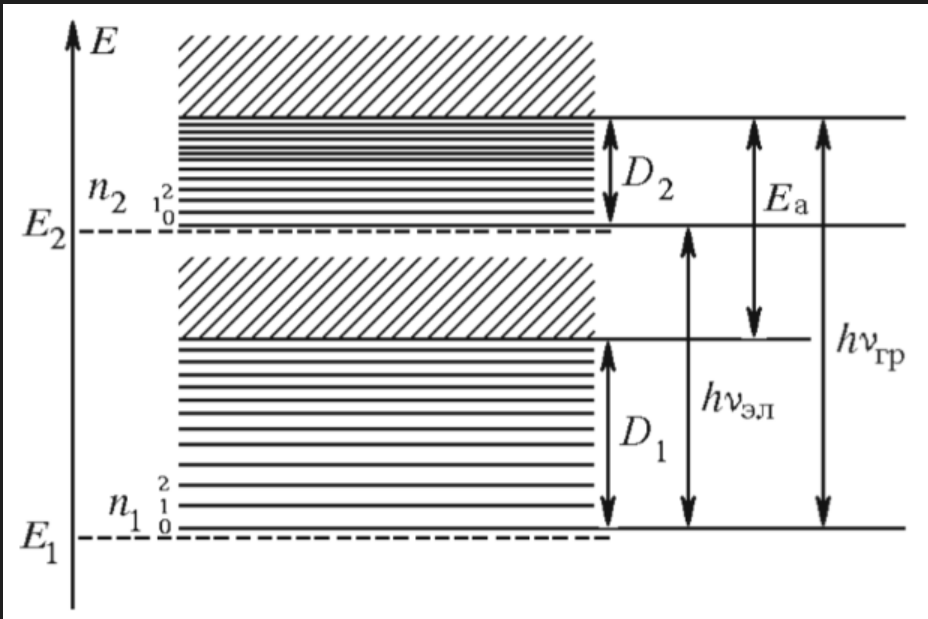
\includegraphics[width=0.6\linewidth]{pics/theory.png}
            \caption{ : электронные и электронно-колебательные уровни двух-атомной молекулы}
            \label{theor}
        \end{figure}

        В данной работе будет исследоваться серия Бальмера атома водорода, в которой электроны совершают переходы с некоторого уровня $n$ на уровень $m = 2$.


        \subsection{Cпектр йода}
        В первом приближении энергия молекулы может быть представлена в виде:
        \begin{equation}
            E=E_e+E_o+E_r,
        \end{equation}
        где $E_e$ -- энергия электронных уровней, $E_o$ -- энергия колебательньных уровней, $E_r$ -- энергия вращательных уровней.

        В настоящей работе рассматриваются оптические переходы, то есть переходы, связанные с излучением фотонов в видимом диапазоне длин волн. Они соответсвтуют переходам между различными электронными состояниями. При этом также происходят изменения вращательного и колебательного состояний, однако в реальности ввиду малости характерных энергий вращательные переходы ненаблюдаемы.

        Более конкретно, изучаются переходы из колебательного состояния с номером $n_1$ освновного электронного уровня с энергией $E_1$ в колебательное состояние с номером $n_2$ на электронный уровень с энергией $E_2$. Энергия таких переходов описывается формулой:
        \begin{equation}
            h \nu_{n_1,n_2}=(E_2-E_1)+h\nu_2(n_2+\dfrac{1}{2})-h \nu_1(n_1+\dfrac{1}{2}),
        \end{equation}
        где $\nu_1$ и $\nu_2$ суть энергии колебательных квантов на электронных уровнях с энергиями $E_1$ и $E_2$.

        При достаточно больших квантовых числах $n_1$ и $n_2$ колебательные уровни переходят в непрерывный спектр, что соответствует диссоциации молекулы. Наименьшая энергия, которую нужно сообщить молекуле в нижайшем колебательном состоянии, чтобы она диссоциировала, называется энергией диссоциации.

        В данной работе определяются энергии диссоциации на первых двух электронных уровнях.
     